\documentclass[10pt,aspectratio=169]{beamer}
%\documentclass[12pt,aspectratio=169]{beamer}

%\mode<presentation>

\usepackage{graphicx}
\usepackage{breqn}
\usepackage{bm}
\usepackage{color}
\usepackage{tabularx}

\usepackage{listings}
\lstset{language=C++}

\usepackage{mathtools}
\DeclarePairedDelimiter\ceil{\lceil}{\rceil}
\DeclarePairedDelimiter\floor{\lfloor}{\rfloor}


%\ifxetex
\usepackage{fontspec}
\newfontfamily{\klavikumfont}{Klavika-Regular.otf}
\selectfont\klavikumfont
%\fi


\usepackage{listings}

%\usepackage[utf8]{inputenc}
\definecolor{bluekeywords}{rgb}{0.63, 0.79, 0.95}
\definecolor{greencomments}{rgb}{0,0.5,0}
\definecolor{redstrings}{rgb}{0.64,0.08,0.08}
\definecolor{xmlcomments}{rgb}{0.5,0.5,0.5}
\definecolor{types}{rgb}{0.17,0.57,0.68}
\lstset{language=C++,
captionpos=b,
%numbers=left,
%numberstyle=\tiny,
frame=single,
showspaces=false,
showtabs=false,
breaklines=true,
showstringspaces=false,
breakatwhitespace=true,
escapeinside={(*@}{@*)},
commentstyle=\color{greencomments},
morekeywords={partial, var, value, get, set},
keywordstyle=\color{bluekeywords},
stringstyle=\color{redstrings},
basicstyle=\ttfamily\small,
}

\usepackage[yyyymmdd]{datetime}
\renewcommand{\dateseparator}{-}

%\usepackage[inline]{asymptote}
\usepackage{asymptote}
\def\asylatexdir{}
\def\asydir{}

\renewcommand{\thefootnote}{\fnsymbol{footnote}}

\def\clap#1{\hbox to 0pt{\hss#1\hss}}
\def\mathllap{\mathpalette\mathllapinternal}
\def\mathrlap{\mathpalette\mathrlapinternal}
\def\mathclap{\mathpalette\mathclapinternal}
\def\mathllapinternal#1#2{\llap{$\mathsurround=0pt#1{#2}$}}
\def\mathrlapinternal#1#2{\rlap{$\mathsurround=0pt#1{#2}$}}
\def\mathclapinternal#1#2{\clap{$\mathsurround=0pt#1{#2}$}}

\def\p{\pause}

\def\({\left(}
\def\){\right)}
\def\[{\left[}
\def\]{\right]}

\def\no#1{\nobreak{#1}} % stop equation breaking in dmath

\begin{asydef}
  // Global Asymptote definitions can be put here.
  import three;
  usepackage("bm");
  texpreamble("\def\V#1{\bm{#1}}");
  // One can globally override the default toolbar settings here:
  // settings.toolbar=true;
\end{asydef}

%\useinnertheme{rectangles} %specifies itemize points to be rectangles
\useoutertheme{default}

\definecolor{darkgreen}{RGB}{0, 100, 0}
\definecolor{brightpurple}{RGB}{160,32,240}

% fg specifies foreground color
% bg specifies background color
% the notation color!x!white mixes the color with 1-x amount of white
%\setbeamercolor{frametitle}{fg=darkgreen!90!black, bg=darkgreen!10!white}
\setbeamercolor{normal text}{fg=white,bg=black}
% defines color of structure elements, e.g., color of text in the
% outline, block titles many more definitions possible. Each element
% predefined by the theme can be overwritten individually

\setbeamerfont{author}{size=\small,series=\bfseries,parent=structure}
\setbeamerfont{frametitle}{family=\fontfamily{cyklop}\selectfont}

\setbeamercolor{background canvas}{bg=white}
%% \usebackgroundtemplate
%% {
%%   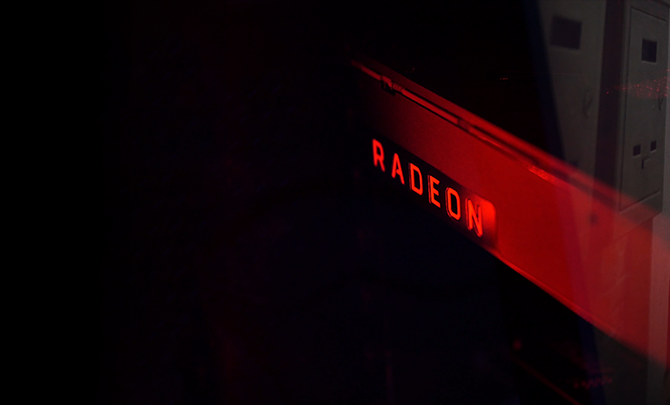
\includegraphics[width=\paperwidth,height=\paperheight]{gpu_background_black.png}
%% }
\pgfdeclareimage[width=\paperwidth]{mybackground}{gpu_background_black.png}
\setbeamertemplate{title page}{
  \begin{picture}(0,0)
    \put(-30,-163){%
      \pgfuseimage{mybackground}
    }
    \put(0,-150){%
      \begin{minipage}[b][45mm][t]{226mm}
        \usebeamerfont{title}{\inserttitle\par}
        \ifx\insertsubtitle\@empty%
        \else%
        {\vskip0.25em%
        \usebeamerfont{subtitle}\usebeamercolor[fg]{subtitle}\insertsubtitle\par}%
        \fi%
        \vskip1cm%              
        \usebeamerfont{author}{\insertauthor\par}
        \usebeamerfont{date}\url{malcolm.roberts@amd.com}\par
        \usebeamerfont{date}\insertdate
      \end{minipage}
    }
  \end{picture}
}

\setbeamerfont{frametitle}{family=\fontspec{Klavika-Regular.otf}}


%------------------------------------------------------------------------
%------------------------------------------------------------------------



\def\thetitle{rocFFT}
\def\thesubtitle{Proposed Optimisations from Runtime Compilation}
\def\theauthor{Malcolm Roberts}
\def\theauthorinstitute{AMD}

\def\presdate{2020-02-14}

\hypersetup{
  pdftitle=\thetitle{} \thesubtitle{},
  pdfauthor=\theauthor{}
}

\title{\thetitle{}}
\subtitle{\thesubtitle{}}
\author{\theauthor{}}
\institute{\theauthorinstitute}
%\date{\presdate}

\setbeamertemplate{frametitle}[default][center]
%\setbeamertemplate{footline}[frame number]
\setbeamertemplate{navigation symbols}{} 

\begin{document}

\klavikumfont

\setbeamertemplate{headline}{}
%\setbeamertemplate{footline}{}

{
  \setbeamercolor{background canvas}{bg=black}
  \setbeamercolor{normal text}{fg=white,bg=black}
  \setbeamercolor{frametitle}{fg=white}
  \setbeamercolor{title}{fg=white}
  \setbeamercolor{alerted text}{fg=white}
  \setbeamercolor{structure}{fg=white}
  \usebeamercolor[fg]{normal text}
  \begin{frame}
    \titlepage
  \end{frame}
}


\setbeamercolor{normal text}{fg=black,bg=white}
\usebeamercolor[fg]{normal text}

\newcolumntype{R}{>{\raggedleft\arraybackslash}X}
\setbeamertemplate{footline}{
   \leavevmode%
   \hbox{%
     \begin{beamercolorbox}[wd=\paperwidth,ht=1ex,dp=1.125ex]{author in head/foot}%
  \begin{tabularx}{\paperwidth}{lR}
    \hfill\insertframenumber/\inserttotalframenumber\hfill\phantom{.}%
    & %
    
\includegraphics[width=0.05\textwidth]{footerlogo}%
    \\%
  \end{tabularx}%
  \end{beamercolorbox}%
   }%
}

\begin{frame}
  \frametitle{Outline}

  \texttt{rocFFT} performance relies on kernels which are
  specific to certain problem size factorization.

  \medskip
  
  In this talk, I will present some optimization plans which would
  greatly benefit from the inclusion of runtime compilation in the
  \texttt{rocFFT} library.

  \bigskip

  These optimizations are as follows:
  
  \bigskip
  \begin{itemize}
  \item Increase Problem Size Coverage for Stockham Kernels
    \medskip
  \item Eliminate Useless Work for Bluestein Kernels
    \medskip
  \item Fuse Kernels for Multidimensional Transforms
  \end{itemize}
  
\end{frame}

\begin{frame}
  \frametitle{Problem Size Coverage}

    FFTs are computed by dividing a problem of length $N$ into smaller
    factors.  These factors are referred to as radices, and
    \texttt{rocFFT} supports radix-2, 3, 5, and 7.  Other combinations
    can also be useful - eg 4 and 8 have nice properties.

    \medskip
    
    Combining kernels to deal with multiple stages of an FFT is
    helpful on the GPU.

    \medskip
    
    \texttt{rocFFT} computes kernels up to the size which fit into
    cache; larger transforms are broken up into multi-stage
    transforms.

    \medskip
    
    For $N \leq 2048$, there are 189 supported sizes.
    
    \medskip

    Adding radix-11 and 13 produces 350 supported sizes.
    
\end{frame}

\begin{frame}
  \frametitle{Problem Size Coverage}

  More radices means more supported lengths.
  
  \begin{center}
    \includegraphics[width=0.7\textwidth]{support_vs_radices.pdf}
  \end{center}
  
\end{frame}

\begin{frame}
  \frametitle{Bluestein algorithm}

  For unsupported problem sizes (eg large primes), one can use
  general-length algorithms such as Bluestein or Radler.

  \medskip

  These methods uses the fact that an FFT can expressed as a convolution.

  \medskip

  A convolution can be computed via an FFT, but needs to be padded with
  zeros from length $N$ to at least length $2N$.

  \medskip

  By padding to some nice size $M \geq 2N$, we can choose $M$ to be a
  supported size.

  \medskip

  The straightforward implementation does a lot of work on zero data.
  
\end{frame}
  
\begin{frame}
  \frametitle{Bluestein algorithm}

  \begin{center}
    \includegraphics[width=\textwidth]{stockham-dit.pdf}
  \end{center}

  \begin{center}
    We could save a lot of work by skipping pointless computations.
  \end{center}
  
\end{frame}
  
\begin{frame}
  \frametitle{Doing More Work with Cached Data}

  Multi-dimensional FFTs are computed by performing batched 1D
  transforms in each direction.

  \medskip

  If the entire problem fits in the cache, we just need one single
  global read/write.

  \medskip

  Larger problems need multiple passes, which are broken down into
  each dimension.

  \medskip

  Repeated trips to and from global memory is an expensive part of the
  FFT algorithm.
  
\end{frame}

\begin{frame}
  \frametitle{Doing More Work with Cached Data}

  The normal way of computing an FFT of size $M\times{}N\times{}P$ is to
  \begin{enumerate}
  \item Read from global
  \item Perform $MN$ length-$P$ transforms
  \item Read from global
  \item Write to global
  \item Perform $MP$ length-$N$ transforms
  \item Read from global
  \item Perform $NP$ length-$M$ transforms
  \item Write to global
  \end{enumerate}

  \begin{center}
Total: 3 global read/writes.
\end{center}

\end{frame}

\begin{frame}
  \frametitle{Doing More Work with Cached Data}

  Suppose $n = \sqrt{N}$, and we can fit $MnP$ values into cache.

  Then, we could
  \begin{enumerate}
  \item Read from global
  \item Perform $MN$ length-$P$ transforms
  \item Perform the $MP$ initial radix-$n$ sub-transforms
  \item Write to global
  \item Read from global
  \item Perform the $MP$ final radix-$n$ sub-transforms
  \item Perform $NP$ length-$M$ transforms
  \item Write to global
  \end{enumerate}
  
  \begin{center}
    Total: 2 global read/writes.
  \end{center}

\end{frame}


\begin{frame}[fragile]
  \frametitle{Conclusion}

  In addition to the three methods described above,
  \begin{itemize}
  \item Increasing supported problem sizes
  \item Skipping pointless computations
  \item Making better use of cached data
  \end{itemize}
  we would like to fuse more kernels to reduce the number of kernels
  required, which would also be aided by runtime computation.

  \medskip

  All of these techniques multiply the number of needed kernels
  combinatorically.


  \medskip

  Most of these optimizations are largely infeasible, or must be reduced
  in scope, if we were to require ahead-of-time compilation.
  
  \medskip
  
  Runtime compilation allows us to continue architecture support while
  improving performance.

  \begin{center}
    Thank you for your time!
  \end{center}
  
\end{frame}

\begin{frame}
  \textbf{Disclaimer}
  \medskip

  \fontsize{8pt}{8pt}\selectfont
  The information presented in this document is for informational
  purposes only and may contain technical inaccuracies, omissions, and
  typographical errors. The information contained herein is subject to
  change and may be rendered inaccurate for many reasons, including
  but not limited to product and roadmap changes, component and
  motherboard version changes, new model and/or product releases,
  product differences between differing manufacturers, software
  changes, BIOS flashes, firmware upgrades, or the like. Any computer
  system has risks of security vulnerabilities that cannot be
  completely prevented or mitigated.  AMD assumes no obligation to
  update or otherwise correct or revise this information. However, AMD
  reserves the right to revise this information and to make changes
  from time to time to the content hereof without obligation of AMD to
  notify any person of such revisions or changes.
  \medskip
 
  THIS INFORMATION IS PROVIDED ``AS IS''. AMD MAKES NO REPRESENTATIONS
  OR WARRANTIES WITH RESPECT TO THE CONTENTS HEREOF AND ASSUMES NO
  RESPONSIBILITY FOR ANY INACCURACIES, ERRORS, OR OMISSIONS THAT MAY
  APPEAR IN THIS INFORMATION. AMD SPECIFICALLY DISCLAIMS ANY IMPLIED
  WARRANTIES OF NON-INFRINGEMENT, MERCHANTABILITY, OR FITNESS FOR ANY
  PARTICULAR PURPOSE. IN NO EVENT WILL AMD BE LIABLE TO ANY PERSON FOR
  ANY RELIANCE, DIRECT, INDIRECT, SPECIAL, OR OTHER CONSEQUENTIAL
  DAMAGES ARISING FROM THE USE OF ANY INFORMATION CONTAINED HEREIN,
  EVEN IF AMD IS EXPRESSLY ADVISED OF THE POSSIBILITY OF SUCH DAMAGES.
  \medskip
    
  Third-party content is licensed to you directly by the third party
  that owns the content and is not licensed to you by AMD.  ALL LINKED
  THIRD-PARTY CONTENT IS PROVIDED “AS IS” WITHOUT A WARRANTY OF ANY
  KIND.  USE OF SUCH THIRD-PARTY CONTENT IS DONE AT YOUR SOLE
  DISCRETION AND UNDER NO CIRCUMSTANCES WILL AMD BE LIABLE TO YOU FOR
  ANY THIRD-PARTY CONTENT.  YOU ASSUME ALL RISK AND ARE SOLELY
  RESPONSIBLE FOR ANY DAMAGES THAT MAY ARISE FROM YOUR USE OF
  THIRD-PARTY CONTENT.
  \medskip

  ATTRIBUTION\\
  © 2021 Advanced Micro Devices, Inc. All rights
  reserved. AMD, the AMD Arrow logo, ROCm, Radeon, Radeon Instinct and
  combinations thereof are trademarks of Advanced Micro Devices,
  Inc. in the United States and/or other jurisdictions. Other names
  are for informational purposes only and may be trademarks of their
  respective owners.
  
\end{frame}
  

\end{document}

% LocalWords:  rocFFT runtime Stockham Bluestein FFTs radices radix
% LocalWords:  eg FFT Radler MnP combinatorically roadmap ROCm Radeon
% LocalWords:  MERCHANTABILITY
